%------------------------------------------------------------------------------
\chapter{Testing hadronic models}
\label{sec:app_2}
%------------------------------------------------------------------------------
This appendix includes the comparison of residuals obtained from alignment using the previously used method and Millepede. The reduced chi-square comparison plots for the two methods were shown earlier.
It also includes the residual versus position plots for the Micromega detectors.
\begin{figure}[h!]
\centering
 \begin{subfigure}[l]{.45\textwidth}
   \centering
   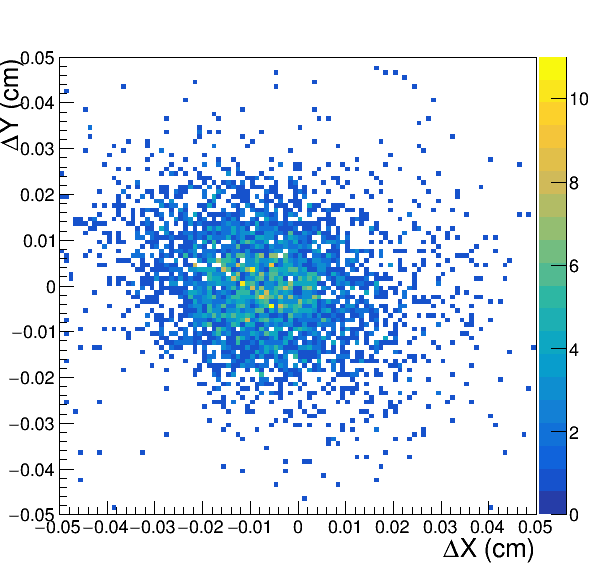
\includegraphics[width=\linewidth]{thesis_figures/alignment/Run_3211_after_prev/square/GEM1.png}

   \caption{GEM1 after previously used method}
   \label{fig:GEM1_after_prev}
 \end{subfigure}
 %\hfill
 \begin{subfigure}[r]{.45\textwidth}
   \centering
   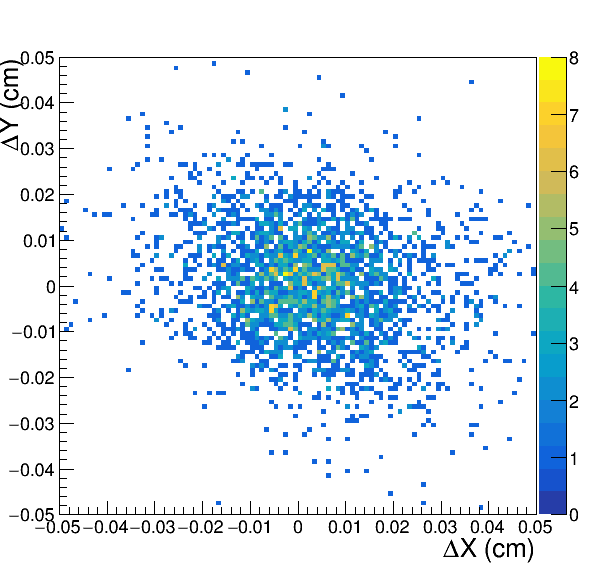
\includegraphics[width=\linewidth]{thesis_figures/alignment/Run_3211_after_millepede/square/GEM1.png}
   \caption{GEM1 after Millepede}
   %\label{fig:GEM1_before}
 \end{subfigure}
 \hfill
 \begin{subfigure}[l]{.45\textwidth}
   \centering
   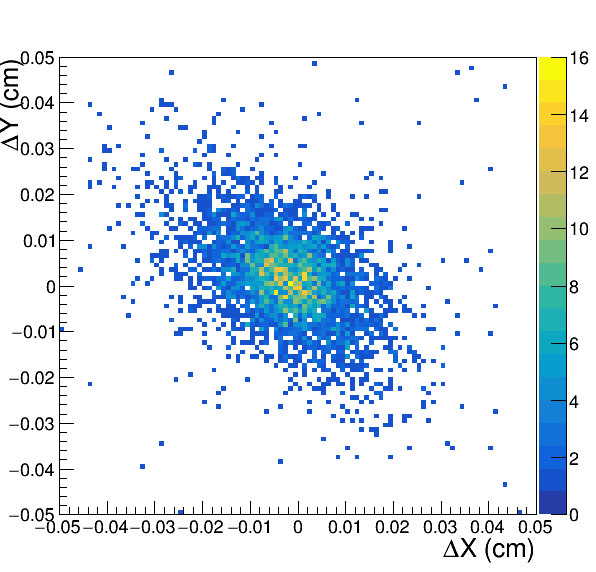
\includegraphics[width=\linewidth]{thesis_figures/alignment/Run_3211_after_prev/square/GEM2.png}
   \caption{GEM2 after previously used method}
   \label{fig:GEM2_after_prev}
 \end{subfigure}
 %\hfill
 \begin{subfigure}[r]{.45\textwidth}
   \centering
   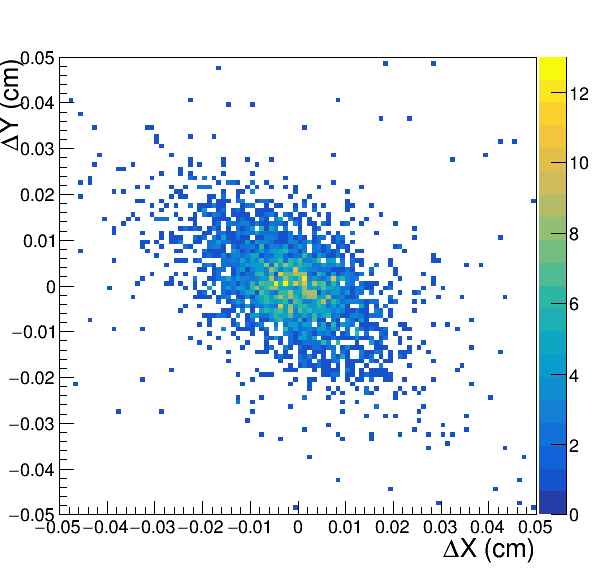
\includegraphics[width=\linewidth]{thesis_figures/alignment/Run_3211_after_millepede/square/GEM2.png}
   \caption{GEM2 after Millepede}
   %\label{fig:GEM2_before}
 \end{subfigure}
 \begin{subfigure}[l]{.45\textwidth}
   \centering
   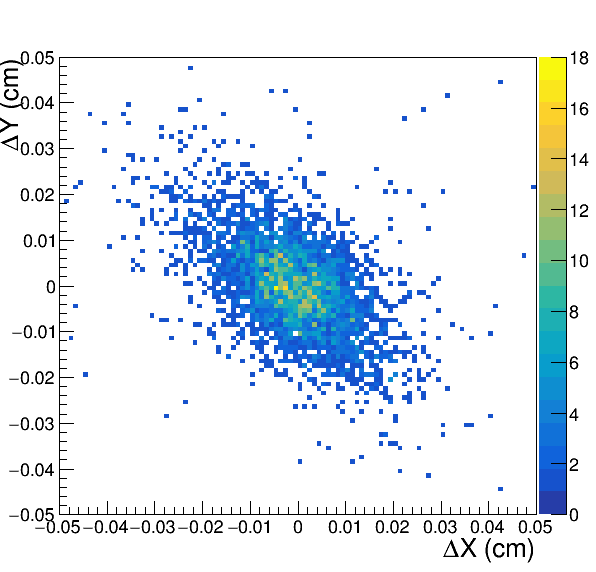
\includegraphics[width=\linewidth]{thesis_figures/alignment/Run_3211_after_prev/square/GEM4.png}

   \caption{GEM4 after previously used method}
   \label{fig:GEM4_after_prev}
 \end{subfigure}
 %\hfill
 \begin{subfigure}[r]{.45\textwidth}
   \centering
   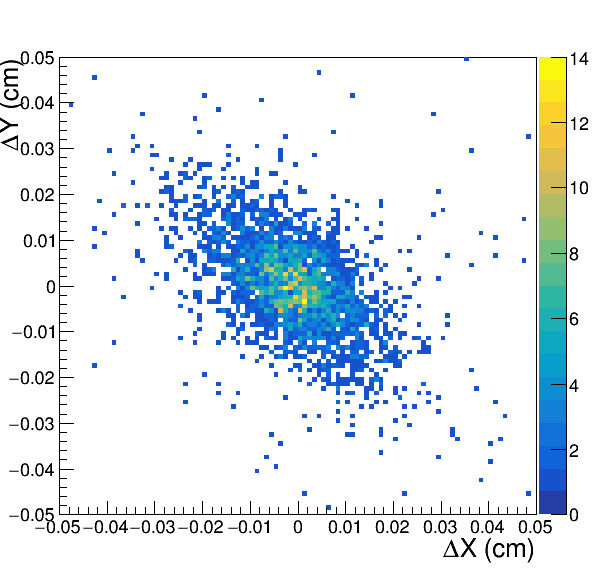
\includegraphics[width=\linewidth]{thesis_figures/alignment/Run_3211_after_millepede/square/GEM4.png}
   \caption{GEM4 after Millepede}
   %\label{fig:GEM4_before}
 \end{subfigure}
 \caption{Residual of GEM detectors.}
\end{figure}

%%%%MICROMEGAS start here

\begin{figure}[h!]
\centering
 \begin{subfigure}[l]{.45\textwidth}
   \centering
   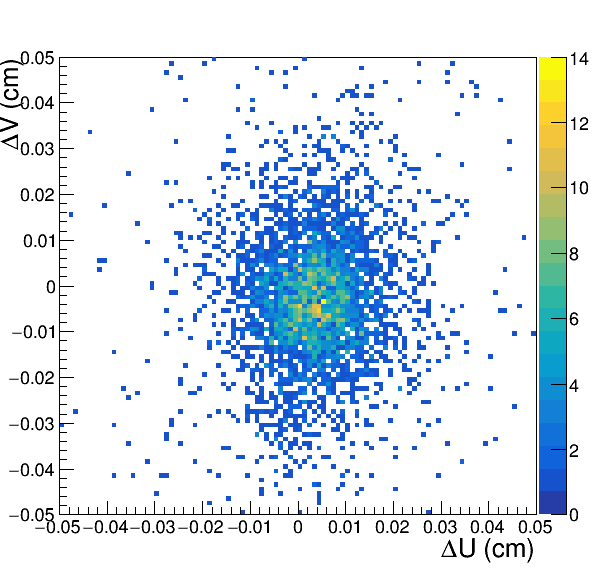
\includegraphics[width=\linewidth]{thesis_figures/alignment/Run_3211_after_prev/square/MX1.png}

   \caption{MM1 after previously used method}
   \label{fig:MX1_after_prev}
 \end{subfigure}
 %\hfill
 \begin{subfigure}[r]{.45\textwidth}
   \centering
   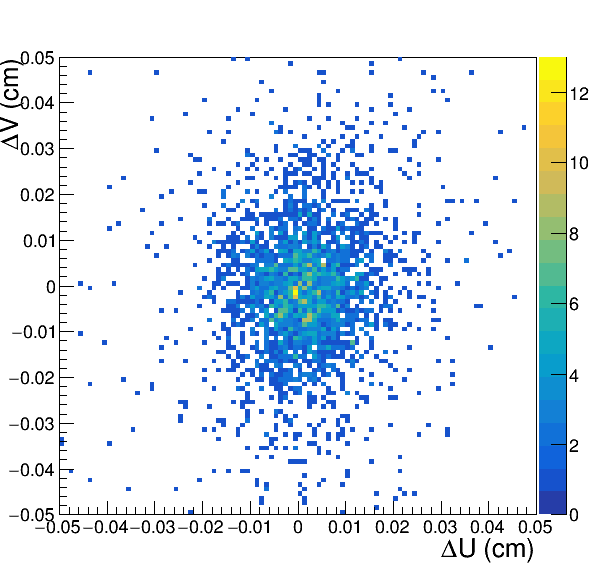
\includegraphics[width=\linewidth]{thesis_figures/alignment/Run_3211_after_millepede/square/MX1.png}
   \caption{MM1 after Millepede}
   %\label{fig:MX1_after}
 \end{subfigure}
 \hfill
 \begin{subfigure}[l]{.45\textwidth}
   \centering
   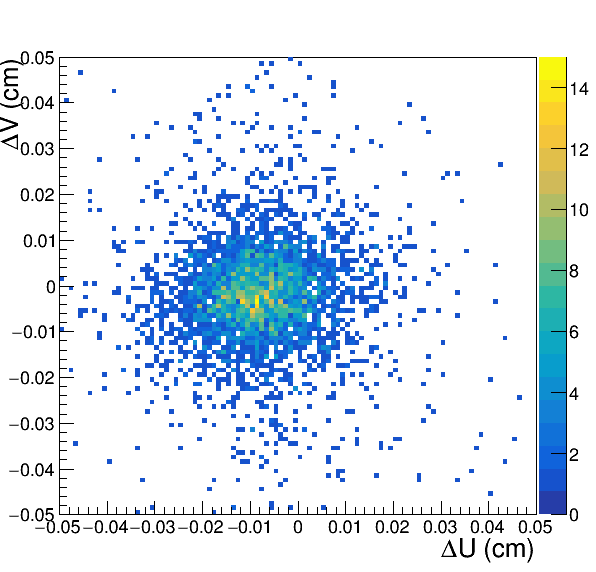
\includegraphics[width=\linewidth]{thesis_figures/alignment/Run_3211_after_prev/square/MX2.png}
   \caption{MM2 after previously used method}
   \label{fig:MX2_after_prev}
 \end{subfigure}
 %\hfill
 \begin{subfigure}[r]{.45\textwidth}
   \centering
   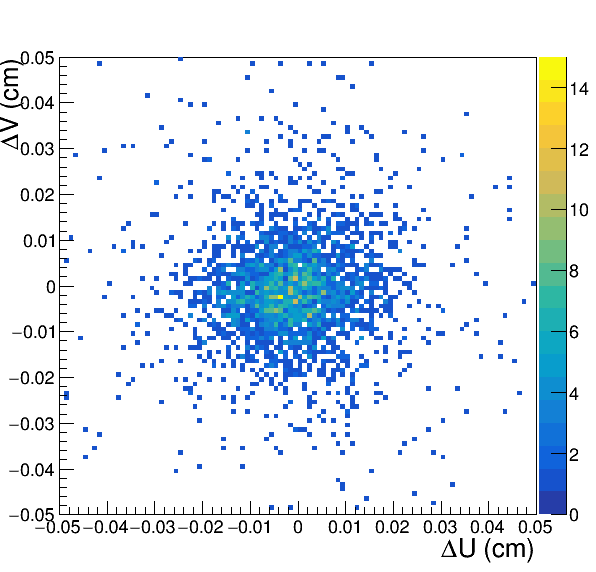
\includegraphics[width=\linewidth]{thesis_figures/alignment/Run_3211_after_millepede/square/MX2.png}
   \caption{MM2 after Millepede}
   %\label{fig:MX2_after}
 \end{subfigure}
 \begin{subfigure}[l]{.45\textwidth}
   \centering
   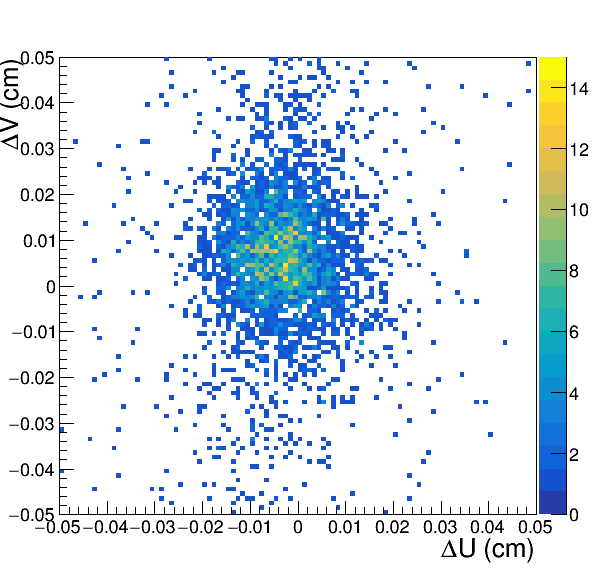
\includegraphics[width=\linewidth]{thesis_figures/alignment/Run_3211_after_prev/square/MX3.png}

   \caption{MM3 after previously used method}
   \label{fig:MX3_after_prev}
 \end{subfigure}
 %\hfill
 \begin{subfigure}[r]{.45\textwidth}
   \centering
   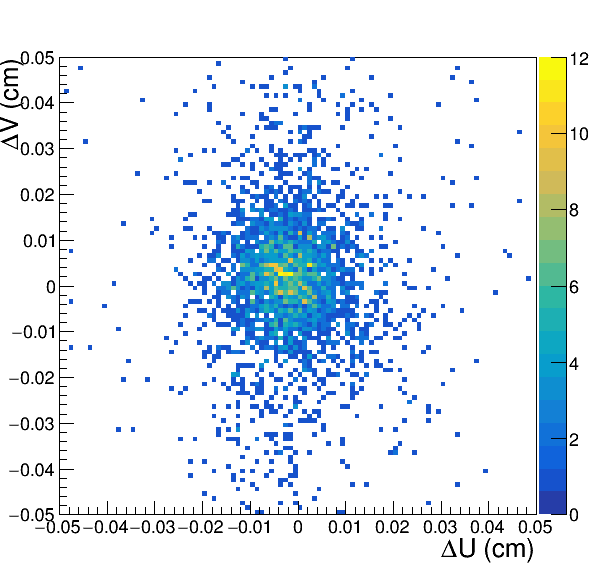
\includegraphics[width=\linewidth]{thesis_figures/alignment/Run_3211_after_millepede/square/MX3.png}
   \caption{MM3 after Millepede}
   %\label{fig:MX3_after}
 \end{subfigure}
 \caption{Residual of Micromega detectors.}
\end{figure}


\begin{figure}[h!]
\centering
 \begin{subfigure}[l]{.45\textwidth}
   \centering
   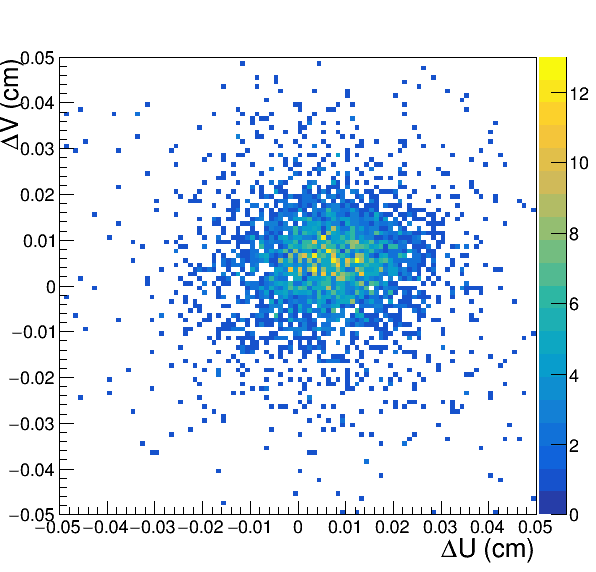
\includegraphics[width=\linewidth]{thesis_figures/alignment/Run_3211_after_prev/square/MX4.png}

   \caption{MM4 after previously used method}
   \label{fig:MX4_after_prev}
 \end{subfigure}
 %\hfill
 \begin{subfigure}[r]{.45\textwidth}
   \centering
   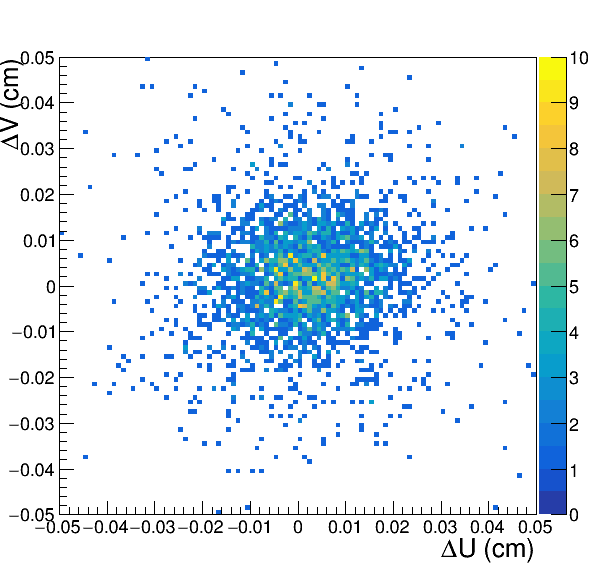
\includegraphics[width=\linewidth]{thesis_figures/alignment/Run_3211_after_millepede/square/MX4.png}
   \caption{MM4 after Millepede}
   %\label{fig:MX4_after}
 \end{subfigure}
 \hfill
 \begin{subfigure}[l]{.45\textwidth}
   \centering
   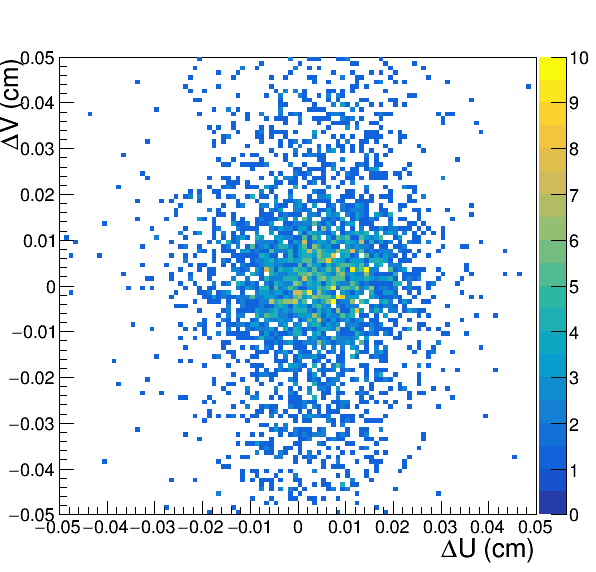
\includegraphics[width=\linewidth]{thesis_figures/alignment/Run_3211_after_prev/square/MX5.png}
   \caption{MM5 after previously used method}
   \label{fig:MX5_after_prev}
 \end{subfigure}
 %\hfill
 \begin{subfigure}[r]{.45\textwidth}
   \centering
   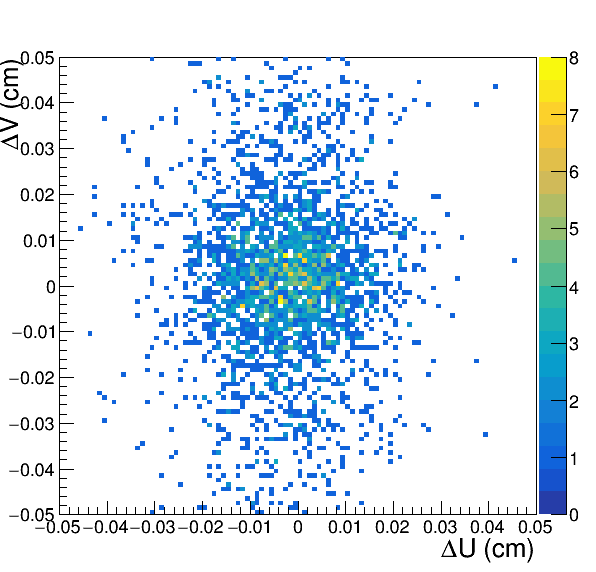
\includegraphics[width=\linewidth]{thesis_figures/alignment/Run_3211_after_millepede/square/MX5.png}
   \caption{MM5 after Millepede}
   %\label{fig:MX5_after}
 \end{subfigure}
 \begin{subfigure}[l]{.45\textwidth}
   \centering
   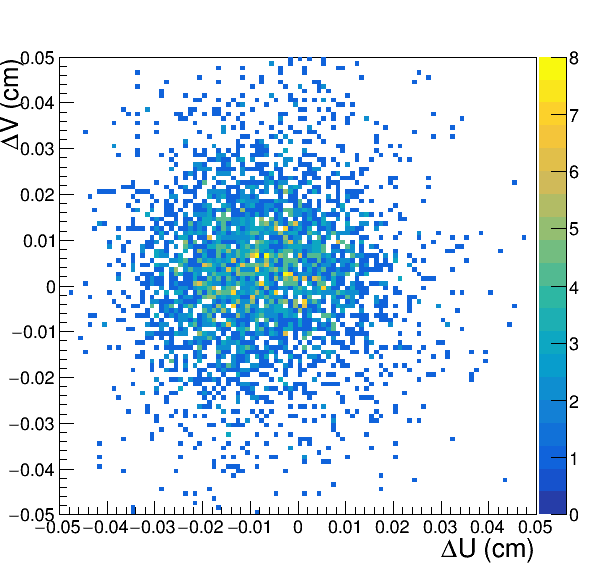
\includegraphics[width=\linewidth]{thesis_figures/alignment/Run_3211_after_prev/square/MX7.png}

   \caption{MM6 after previously used method}
   \label{fig:MX6_after_prev}
 \end{subfigure}
 %\hfill
 \begin{subfigure}[r]{.45\textwidth}
   \centering
   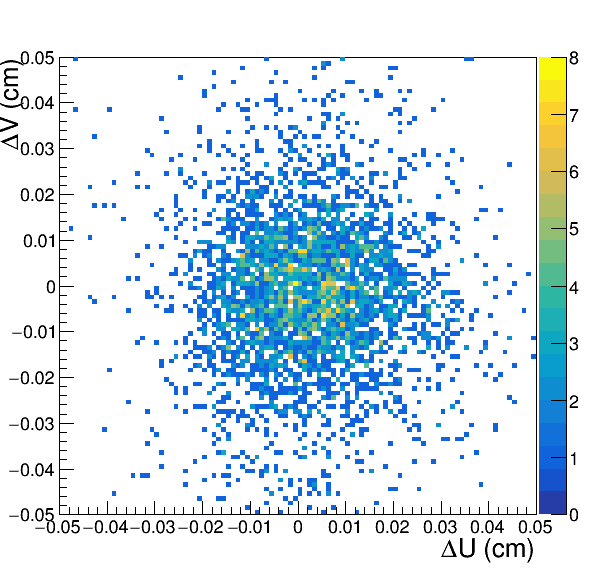
\includegraphics[width=\linewidth]{thesis_figures/alignment/Run_3211_after_millepede/square/MX7.png}
   \caption{MM6 after Millepede}
   %\label{fig:MX6_after}
 \end{subfigure}
 \caption{Residual of Micromega detectors.}
\end{figure}

%%micromegas%

\begin{figure}[h!]
\centering
 \begin{subfigure}[l]{.45\textwidth}
   \centering
   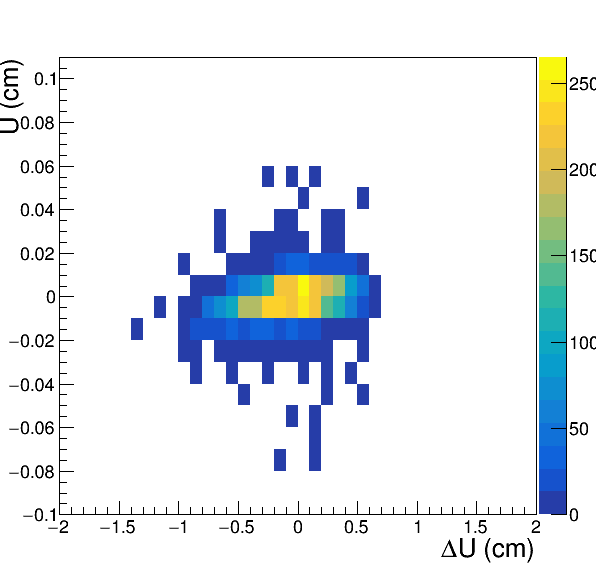
\includegraphics[width=\linewidth]{thesis_figures/alignment/Run_3211_T/rotMX1U_after_millepede_T.png}
   \caption{MM1 U plane}
   %\label{fig:MX1X_before}
 \end{subfigure}
 %\hfill
 \begin{subfigure}[r]{.45\textwidth}
   \centering
   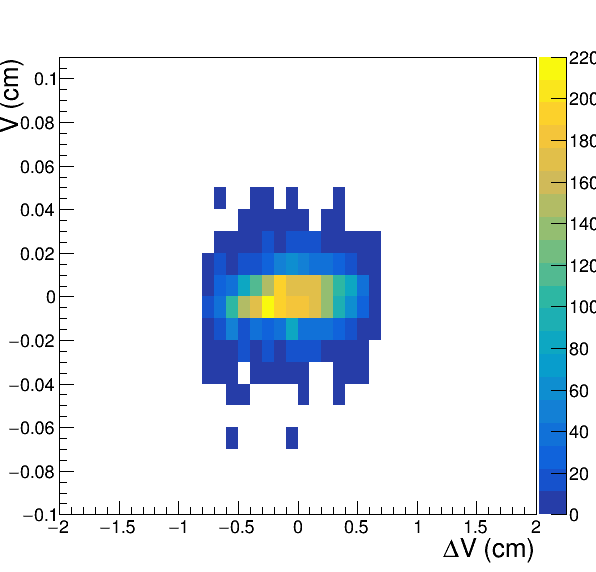
\includegraphics[width=\linewidth]{thesis_figures/alignment/Run_3211_T/rotMX1V_after_millepede_T.png}
   \caption{MM1 V plane}
   %\label{fig:MX1Y_before}
 \end{subfigure}
 \hfill
 \begin{subfigure}[l]{.45\textwidth}
   \centering
   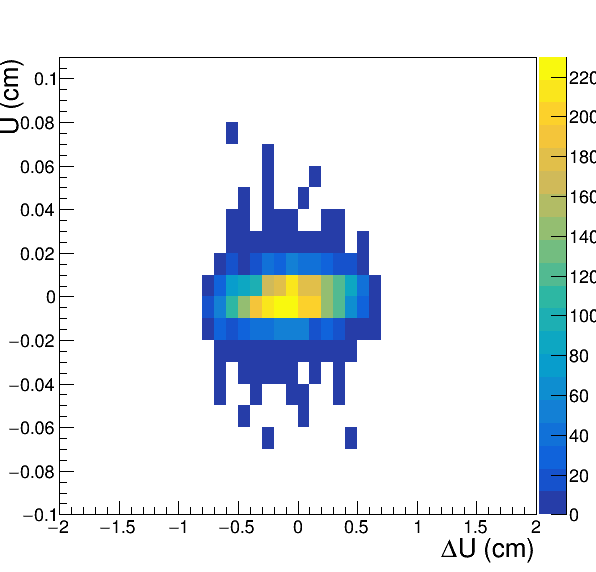
\includegraphics[width=\linewidth]{thesis_figures/alignment/Run_3211_T/rotMX2U_after_millepede_T.png}
   \caption{MM2 U plane}
   %\label{fig:GEM2X_before}
 \end{subfigure}
 \begin{subfigure}[r]{.45\textwidth}
   \centering
   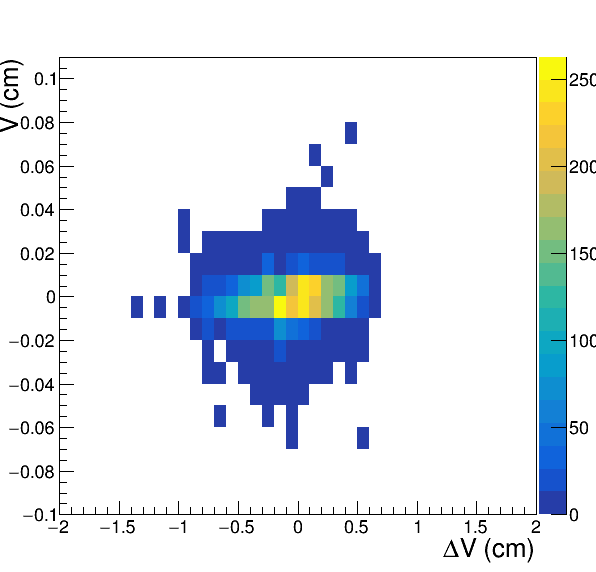
\includegraphics[width=\linewidth]{thesis_figures/alignment/Run_3211_T/rotMX2V_after_millepede_T.png}
   \caption{MM2 V plane}
   %\label{fig:GEM2Y_before}
 \end{subfigure}
 \hfill
 \begin{subfigure}[l]{.45\textwidth}
   \centering
   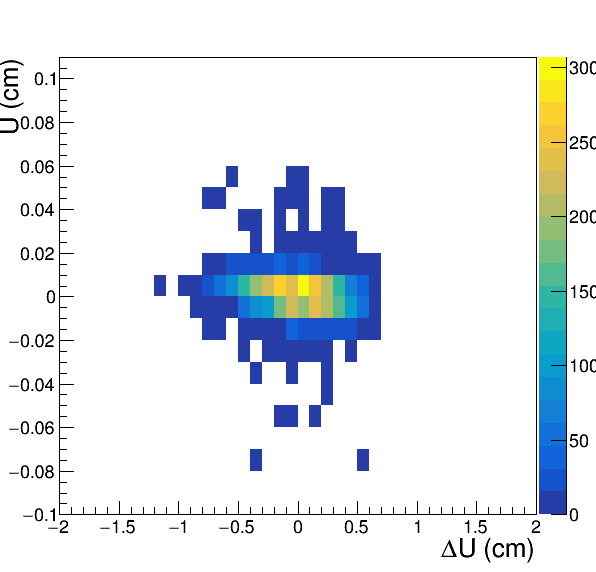
\includegraphics[width=\linewidth]{thesis_figures/alignment/Run_3211_T/rotMX3U_after_millepede_T.png}
   \caption{MM3 U plane}
   %\label{fig:MX1 X plane}
 \end{subfigure}
 %\hfill
 \begin{subfigure}[r]{.45\textwidth}
   \centering
   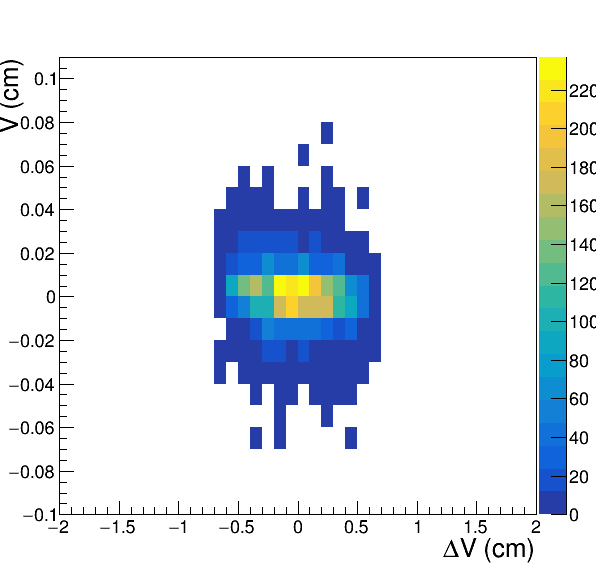
\includegraphics[width=\linewidth]{thesis_figures/alignment/Run_3211_T/rotMX3V_after_millepede_T.png}
   \caption{MM3 V plane}
   %\label{fig:GEM4Y_before}
 \end{subfigure}
 \caption{Residual vs position for Micromega detectors}
 \label{fig:res_vs_pos_MX}
\end{figure}

\begin{figure}[t!]
\begin{subfigure}[l]{.45\textwidth}
  \centering
  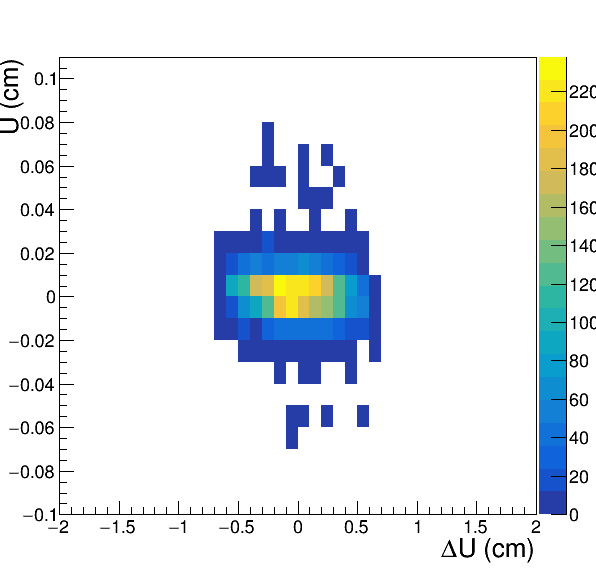
\includegraphics[width=\linewidth]{thesis_figures/alignment/Run_3211_T/rotMX4U_after_millepede_T.png}
  \caption{MM4 U plane}
  %\label{fig:GEM4X_before}
\end{subfigure}
%\hfill
\begin{subfigure}[r]{.45\textwidth}
  \centering
  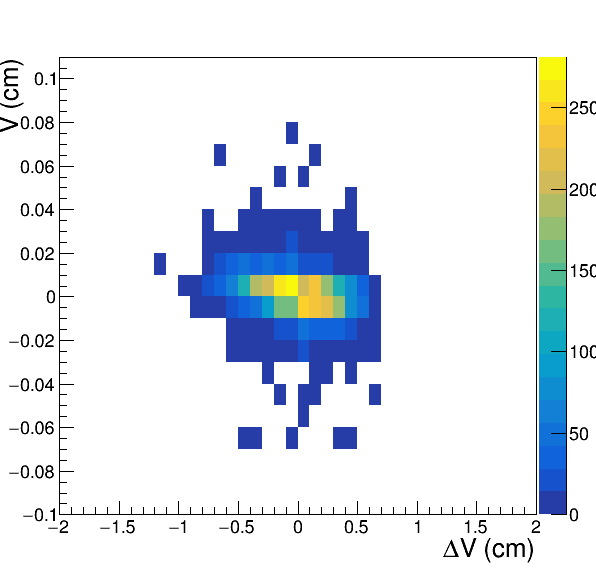
\includegraphics[width=\linewidth]{thesis_figures/alignment/Run_3211_T/rotMX4V_after_millepede_T.png}
  \caption{MM4 V plane}
  %\label{fig:GEM4Y_before}
\end{subfigure}
\caption{ Residual vs position for MM4}
\end{figure}
%%% Local Variables:
%%% mode: latex
%%% TeX-master: "../mythesis"
%%% End:
